\documentclass[10pt,conference, compsocconf]{IEEEtran}

\usepackage{amsfonts}
\usepackage{amssymb,amsmath}
\usepackage{hyperref}
\usepackage{algpseudocode}
\usepackage{graphicx}
\usepackage{anyfontsize}   % for fontsize and selectfont command
\usepackage{array}         % better padding of cell content of tabulars
\usepackage[skip=2pt,font=footnotesize]{caption}

\usepackage{tikz}       % for flowcharts
\usetikzlibrary{shapes, arrows}

\newsavebox{\ieeealgbox}
\newenvironment{boxedalgorithmic}
  {\begin{lrbox}{\ieeealgbox}
   \begin{minipage}{\dimexpr\columnwidth-2\fboxsep-2\fboxrule}
   \begin{algorithmic}}
  {\end{algorithmic}
   \end{minipage}
   \end{lrbox}\noindent\fbox{\usebox{\ieeealgbox}}}

\begin{document}

\title{A shuffled complex evolution algorithm for
the multidimensional knapsack problem}

\author{\IEEEauthorblockN{Marcos Daniel Valad\~ao Baroni}
\IEEEauthorblockA{ Departamento de Inform\'atica\\
Universidade Federal do Esp\'irito Santo\\
Vit\'oria, Esp\'irito Santo, Brazil\\
Email: mbaroni@ninfa.inf.ufes.br }
\and
\IEEEauthorblockN{Fl\'avio Miguel Varej\~ao}
\IEEEauthorblockA{ Departamento de Inform\'atica\\
Universidade Federal do Esp\'irito Santo\\
Vit\'oria, Esp\'irito Santo, Brazil\\
Email: fvarejao@ninfa.inf.ufes.br }
}

\maketitle

\begin{abstract}
This work addresses the application of
a population based evolutionary algorithm
called shuffled complex evolution (SCE) in the multidimensional knapsack
problem.
The SCE regards a natural evolution happening simultaneously in independent communities.
The performance of the SCE algorithm is verified through computational experiments
using well-known problems from literature and randomly generated problem as well.
The SCE proved to be very effective in finding good solutions demanding a
very small amount of processing time.

\end{abstract}
\IEEEpeerreviewmaketitle

\section{Introduction}
\label{sec:intro}

The Multidimensional Knapsack Problem (MKP) is a strongly NP-hard combinatorial
optimization problem which can be viewed as a resource allocation problem and
defined as follows:

\begin{align*}
  \text{maximize} & \sum_{j=1}^n p_j x_j \\
  \text{subject to} & \sum_{j=1}^n w_{ij} x_j \leqslant c_i \quad i \in \{1, \ldots, m\}\\
   & x_j \in \{0, 1\}, \quad j \in \{1, \ldots, n\}.
\end{align*}

% Define the MKP
The problem can be interpreted as a set of $n$ items with profits $p_j$
and a set of $m$ resources with capacities $c_i$.
Each item $j$ consumes an amount $w_{ij}$ from each resource $i$, if selected.
The objective is to select a subset of items with maximum total profit,
not exceeding the defined resource capacities.
The decision variable $x_j$ indicates if $j$-th item is selected.

The multidimensional knapsack problem can be applied on budget planning 
scenarios, subset project selections, cutting stock problems, task scheduling,
allocation of processors and databases in distributed computer programs.
The problem is a generalization of the well-known knapsack problem (KP) in which
$m = 1$.

The MKP is a NP-Hard problem significantly harder to solve in practice than the KP.
Despite the existence of a fully polynomial approximation scheme (FPAS) for the KP,
finding a FPAS for the MKP is NP-hard for $m \geqslant 2$~\cite{magazine1984note}.
Due its simple definition but challenging difficulty the MKP is often used to
to verify the efficiency of novel metaheuristics.

%A metaheuristic is a set of concepts that can be used to define heuristic methods
%that can be applied to a wide set of different problems.
%In other words, a metaheuristic can be seen as a general algorithmic framework which can be applied to
%different optimization problems with relatively few modifications to make them adapted to a specific problem.”

In this paper we address the application of a metaheuristic called
shuffled complex evolution (SCE) to the multidimensional knapsack problem.
The SCE is a metaheuristic, proposed by Duan in \cite{duan1992effective},
which combines the ideas of a controlled random search with the concepts
of competitive evolution and shuffling.
The SCE algorithm has been successfully used to solve several problems
like flow shop scheduling~\cite{zhao2014shuffled} and project management~\cite{elbeltagi2007modified}.

The reminder of the paper is organized as follows:
Section~\ref{sec:sce} presents the shuffled complex evolution algorithm
and proposes its application on the multidimensional knapsack problem.
Section~\ref{sec:exp} comprises several computational experiments.
In section~\ref{sec:conc} we make our concluding remarks about the experimental
results.

\section{The shuffled complex evolution for the MKP}
\label{sec:sce}

%The SFLA is a metaheuristic to solve discrete and combinatorial problems
%based on the memetics of living beings and recalls the behavior of a
%group of frogs searching for the location that has the maximum amount of available food.
%In the following subsections we present the concepts of SCE and PSO to finally
%present the shuffled frog leaping algorithm.

%\label{sec:sfla-mkp}

The shuffled complex evolution is a population
based evolutionary optimization algorithm that regards a natural 
evolution happening simultaneously in independent communities.
The algorithm works with a population partitioned in $N$ complexes, each one
having $M$ individuals.
In the next Subsection the SCE is explained in more details.
In the later Subsection the application of SCE to the multidimensional knapsack
problem is considered.
% In the SCE the population is partitioned into communities (complexes), each of which
% will evolve independently through a number of evolving steps.
% In each evolving step a subset of the complex (subcomplex) is selected as potencial group of
% parents.

%To avoid been trapped in local optimum a new offspring can be occasionally taken
%from a random location of the feasible space and introduced to the complex.

\subsection{The shuffled complex evolution}
In the SCE a population of $N*M$ individuals is randomly taken from the
feasible solution space.
After this initializing the population is sorted by descending order according
to their fitness and the best global solution is identified.
The entire population is then partitioned (shuffled) into $N$ complexes,
each containing $M$ individuals.
In this shuffling process the first individual goes to the first complex, the second
individual goes to the second complex, individual $N$ goes to $N$-th complex,
individual $M+1$ goes back to the first complex, etc.

The next step after shuffling the complexes is to evolve each complex through
a given fixed amount of $K'$ steps.
In each step a subcomplex of $P$ individuals is selected from the
complex using a triangular probability distribution, where the $i$-th individual
has a probability $p_i = \frac{2(n+1-i)}{n(n+1)}$ of being selected.
The use of triangular distribution is intended to prioritize individuals with
better fitness, supporting the algorithm convergence rate.

After the selection of the subcomplex, its worst individual is identified to
be replaced by a new generated solution.
This new solution is generated by the crossing of the worst individual and an
other individual with better fitness.
At first the best individual of the subcomplex is considered for the crossing.
If the new solution is not better than the worst one, the best individual
of the complex is considered for a crossing.
If the latter crossing did not result in any improvement, the best individual
of whole population is considered.
Finally, if all the crossing steps couldn't generate a better individual,
the worst individual of the subcomplex is replaced by a new random solution taken
from the feasible solution space.
This last step is important to prevent the algorithm becoming trapped in local minima.
Fig.~\ref{fig:flow2} presents the procedure described above in a flowchart diagram.

After evolving all the $N$ complexes the whole population is again
sorted by descending and the process continues until a stop condition is satisfied.
Fig.~\ref{fig:flow1} shows the SCE algorithm in a flowchart diagram.

\begin{figure}
  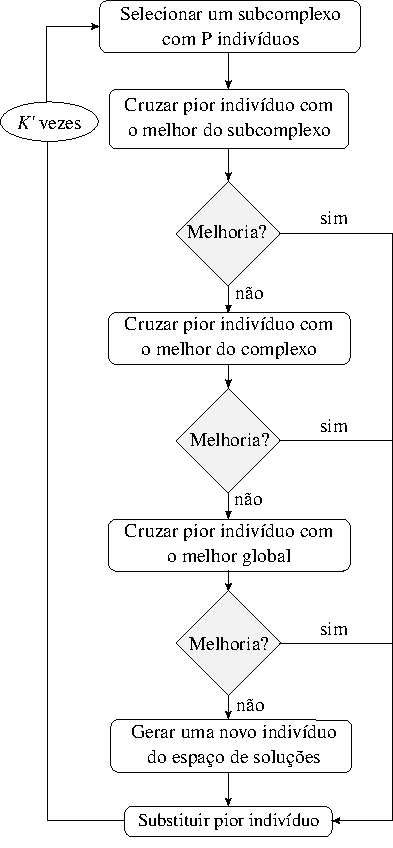
\includegraphics{imgs/flow2}
  \caption{The evolving stage of SCE for a single complex.}
  \label{fig:flow2}
\end{figure}

\begin{figure}
  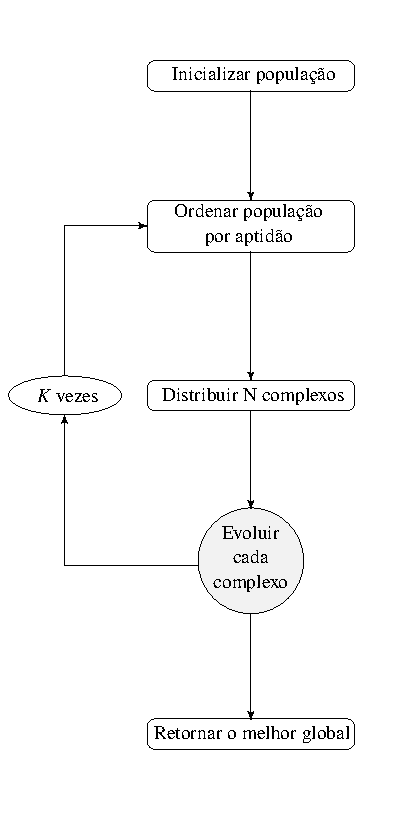
\includegraphics{imgs/flow1}
  \caption{The shuffled complex evolution algorithm.}
  \label{fig:flow1}
\end{figure}


\subsection{The shuffled complex evolution for the MKP}

As it can be noted in its description the SCE is easly applied to any
optimization problem.
The only steps needed to be specified is (a) the creation of a new random
solution and (b) the crossing procedure of two solutions.
These two procedures are respectively presented by Fig.~\ref{alg:new} and
Fig.~\ref{alg:cross}.

\begin{figure}
\begin{algorithmic}[1]
  \Procedure{New random solution}{}
    \State $v \leftarrow $ shuffle($1, 2, \ldots, n$)
	\State $s \leftarrow \emptyset$ \Comment{empty solution}
    \For{$ i \leftarrow 1:n$ }
	  \State $s \leftarrow s \cup \{v_i\}$ \Comment{adding item}
	  \If{ $s$ is not feasible} \Comment{checking feasibility}
	    \State $s \leftarrow s - \{v_i\}$
      \EndIf
	\EndFor
  \State return $s$
  \EndProcedure
\end{algorithmic}
\caption{Generation of a new random solution for the MKP.}
\label{alg:new}
\end{figure}

To construct a new random solution (Fig.~\ref{alg:new}) the items are
at first shuffled in random order and stored in a list (line 2).
A new empty solution is then defined (line 3).
The algorithm iteratively tries to fill the solution's knapsack with 
the an item taken from the list (lines 4-9).
The feasibility of the solution is then checked: if the item insertion let
the solution unfeasible (line 6) its removed from knapsack (line 7).
After trying to place all available items the new solution is returned.

\begin{figure}
\begin{algorithmic}[1]
  \Procedure{Crossing}{$x^w:$ worst individual, $x^b:$ better individual, $c$}
    \State $v \leftarrow $ shuffle($1, 2, \ldots, n$)
    \For{$ i \leftarrow 1:c$ }
	  \State $j \leftarrow v_i$
	  \State $x^w_j \leftarrow x^b_j$ \Comment{gene carriage}
	\EndFor
	\If{$s^w$ is not feasible}
	  \State repair $s^w$
	\EndIf
	\State update $s^w$ fitness
  \State return $s^w$
  \EndProcedure
\end{algorithmic}
\caption{Crossing procedure used on SCE algorithm.}
\label{alg:cross}
\end{figure}

The crossing procedure (Fig.~\ref{alg:cross}) takes as input the worst
solution taken from the subcomplex $x^w = (x^w_1, x^w_2, \ldots, x^w_n$),
the selected better solution $x_b = (x^b_1, x^b_2, \ldots, x^b_n$)
and the number $c$ of genes that will be carried from the better solution.
The $c$ parameter will control how similar the worst individual will be from the
given better individual.
At first the items are shuffled in random order and stored in a list (line 2).
Then $c$ randomly chosen genes are carried from the better individual to the worst
individual (line 5).
At the end of steps the feasibility of the solution is checked (line 7) and
the solution is repaired if needed.
The repair stage is a greedy procedure that iteratively removes the item that less
decreases the objective function.
Finally the fitness of the generated solution is updated (line 10) and
returned (line 11).

%\begin{algorithmic}
%  \Procedure{The SCE for the MKP}{$\vec{p}, W, \vec{b}$}
%    \State Inicialize population
%    \For{$ i \leftarrow 1:K$ }
%	  \State Sort population by fitness
%	  \State $s_{gb} \leftarrow$ Global best individual
%	  \State Shuffle complexes
%      \For{ each complex }
%	    \State $s_{cb} \leftarrow$ Complex best individual
%        \For{$ k \leftarrow 1:K'$ }
%		  \State Select a subcomplex of $P$ individuals
%          \State $s_w \leftarrow$ worst individual of subcomplex
%          \State $s_b \leftarrow$ best individual of subcomplex
%		  \State $s_{new} \leftarrow s_w \otimes s_b$
%		  \If{ $fitness(s_{new}) > s_w$}
%		    \State $s_w \leftarrow s_{new}$
%		  \Else
%		    \State $s_{new} \leftarrow s_w \otimes s_{cb}$
%		    \If{ $fitness(s_{new}) > s_w$}
%		      \State $s_w \leftarrow s_{new}$
%			\Else
%		      \State $s_{new} \leftarrow s_w \otimes s_{gb}$
%		      \If{ $fitness(s_{new}) > s_w$}
%		        \State $s_w \leftarrow s_{new}$
%		      \Else
%			    \State $s_w \leftarrow$ new random solution
%			  \EndIf
%		    \EndIf
%		  \EndIf
%        \EndFor
%      \EndFor
%    \EndFor
%	\State $s_gb \leftarrow$ Global best individual
%	\State Return $s_gb$
%  \EndProcedure
%\end{algorithmic}

%\begin{algorithmic}
%  \Procedure{New random MKP solution}{$\vec{p}, W, \vec{b}$}
%    \State $\vec{v} \leftarrow $ shuffle$(1, 2, \ldots, n)$
%	\State $s \leftarrow \emptyset $
%    \For{$ i \leftarrow 1:niter$ }
%	  \If{$ s \cup \{v[i]\} is feasible$}
%	    \State $s \leftarrow s \cup \{v[i]\}$
%	  \EndIf
%    \EndFor
%  \EndProcedure
%\end{algorithmic}

\section{Computational experiments}
\label{sec:exp}

For the computational experiments a batch of tests was driven to find the best
parameters for the problem.
Afterwards two main tests was considered:
(a) using the well-known set of problems defined by Chu and Beasley (\cite{Chu-Beasley-1998})
and (b) a large set of randomly generated instances using uniform distribution.

\subsection{The Chu-Beasley instances}

The set of MKP instances provided by Chu and Beasley was generated using a
procedure suggested by Freville and Plateau~\cite{freville1994efficient}, which
attempts to generate instances hard to solve.
The number of constraints $m$ varies among $5$, $10$ and $30$, and the number
of variables $n$ varies among $100$, $250$ and $500$.

The $w_{ij}$ were integer numbers drawn from the discrete uniform distribution
$U(0, 1000)$.
The capacity coefficient $c_i$ were set using
$b_i = \alpha\sum_{j=1}^{n} w_{ij}$ where $\alpha$ is a tightness ratio and
varies among $0.25$, $0.5$ and $0.75$.
For each combination of $(m,n,\alpha)$ parameters, $10$ random problems was generated,
totaling $270$ problems.
The profit $p_j$ of the items were correlated to $w_{ij}$ and generated as follows:
\begin{displaymath}
  p_j = \sum_{i=1}^m \frac{w_{ij}}{m} + 500q_j \qquad j = 1, \ldots, n
\end{displaymath}

\subsection{The set of random instances}

The second set of instances is composed by problems generated using a similar
setup.
The only differences is that the profit $p_j$ is also drawn from a discrete uniform
distribution $U(0, 1000)$.
For each combination of $(m, n, \alpha)$ parameter, $600$ random problems was
generated, totaling $16200$ problems.

\subsection{Experimental results}

All the experiments was run on a Intel$^R$ Core i5-3570 CPU @3.40GHz computer
with 4GB of RAM.
The SCE algorithm for MKP was implemented in C programming language.
For the set of random instance all best known solution was found by the solver
SCIP 3.0.1 running for at least 10 minutes.

After a previous test batch the following parameters for SCE was defined and used
in all executions of SCE:
\begin{itemize}
  \item $N = 20$: number of complexes;
  \item $M = 20$: number of individuals in each complex;
  \item $P = 5$: number of individuals in each subcomplex;
  \item $K = 300$: number of algorithm iterations;
  \item $K' = 20$: number of iterations used in the complex evolving process;
  \item $c = n/5$: number of genes carried from parent in crossing process.
\end{itemize}

Table~\ref{tab:chu} shows the performance of the SCE on the Chu-Beasley set of instance.
Each instance in the set was executed 10 times on SCE.
The \textit{SCE time} column shows the average execution time of SCE algorithm.
The \textit{gap} column shows the average ratio of the solution found by SCE and
the best known solution of each instance.
It can be observed that the SCE has a fast convergence speed, achieving high
quality solutions in few seconds.

\begin{table}
{
\renewcommand{\arraystretch}{1.5}%
\fontsize{8.5pt}{1em}\selectfont 
\begin{center}
\begin{tabular}{|r|r|r|rr|} \hline
\textbf{n}   & \textbf{m}  & \textbf{$\alpha$} & \textbf{SCE time (s)} & \textbf{gap (\%)} \\ \hline
100 & 5 & 0.25 & 0.79 & 96.5 \\
    &   & 0.5 & 0.81 & 97.4 \\
    &   & 0.75 & 0.83 & 98.9 \\ \cline{2-5}
    & 10 & 0.25 & 0.75 & 95.7 \\
    &    & 0.5 & 0.93 & 96.7 \\
    &    & 0.75 & 0.89 & 98.5 \\ \cline{2-5}
    & 30 & 0.25 & 1.01 & 95.4 \\
    &    & 0.5 & 1.07 & 96.4 \\
    &    & 0.75 & 0.99 & 98.2 \\ \cline{2-5}
    & \multicolumn{3}{r}{\textbf{average gap}}  & $\bf 97.1$  \\ \hline \hline
\textbf{n}   & \textbf{m}  & \textbf{$\alpha$} & \textbf{SCE time (s)} & \textbf{gap (\%)} \\ \hline
250 & 5 & 0.25 & 1.72 & 93.2 \\
    &   & 0.5 & 1.75 & 94.9 \\
    &   & 0.75 & 1.78 & 97.6 \\ \cline{2-5}
    & 10 & 0.25 & 1.84 & 93.1 \\
    &    & 0.5 & 1.84 & 94.6 \\
    &    & 0.75 & 1.81 & 97.2 \\ \cline{2-5}
    & 30 & 0.25 & 2.21 & 93.2 \\
    &    & 0.5 & 2.21 & 94.2 \\
    &    & 0.75 & 2.31 & 96.6 \\ \cline{2-5}
    & \multicolumn{3}{r}{\textbf{average gap}}  & $\bf 95.0$  \\ \hline \hline
\textbf{n}   & \textbf{m}  & \textbf{$\alpha$} & \textbf{SCE time (s)} & \textbf{gap (\%)} \\ \hline
500 & 5 & 0.25 & 3.16 & 91.4 \\
    &   & 0.5 & 3.18 & 93.4 \\
    &   & 0.75 & 3.34 & 96.4 \\ \cline{2-5}
    & 10 & 0.25 & 3.39 & 91.7 \\
    &    & 0.5 & 3.37 & 93.1 \\
    &    & 0.75 & 3.44 & 96.2 \\ \cline{2-5}
    & 30 & 0.25 & 3.83 & 91.4 \\
    &    & 0.5 & 3.90 & 92.6 \\
    &    & 0.75 & 3.99 & 96.0 \\ \cline{2-5}
    & \multicolumn{3}{r}{\textbf{average gap}}  & $\bf 93.6$  \\ \hline
\end{tabular}
\end{center}
}
 \caption{SCE performance on Chu-Beasley problems.}
 \label{tab:chu}
\end{table}

\begin{table}
{
\renewcommand{\arraystretch}{1.5}%
\fontsize{8.5pt}{1em}\selectfont 
\begin{center}
\begin{tabular}[c]{|r|r|r|rrr|} \hline
\textbf{n}   & \textbf{m}  & \textbf{$\alpha$}    &\textbf{SCIP time (s)}& \textbf{SCE time (s)} & \textbf{gap (\%)} \\ \hline
100 & 10 & 0.25 & $  0.93$ & $  0.41$  & $98.3$ \\
    &    & 0.50 & $  0.28$ & $  0.39$  & $99.3$ \\
    &    & 0.75 & $  0.09$ & $  0.37$  & $99.8$ \\ \cline{2-6}
    & 20 & 0.25 & $  3.15$ & $  0.41$  & $98.2$ \\
    &    & 0.50 & $  0.71$ & $  0.40$  & $99.3$ \\
    &    & 0.75 & $  0.16$ & $  0.37$  & $99.8$ \\ \cline{2-6}
    & 30 & 0.25 & $  7.26$ & $  0.42$  & $98.3$ \\
    &    & 0.50 & $  1.47$ & $  0.42$  & $99.3$ \\
    &    & 0.75 & $  0.25$ & $  0.38$  & $99.8$ \\ \cline{2-6}
    & \multicolumn{4}{r}{\textbf{average gap}}  & $\bf 99.1$  \\ \hline \hline
\textbf{n}   & \textbf{m}  & \textbf{$\alpha$}    &\textbf{SCIP time (s)}& \textbf{SCE time (s)} & \textbf{gap (\%)} \\ \hline
250 & 10 & 0.25 & $ 58.20$ & $  1.10$  & $97.2$ \\
    &    & 0.50 & $  8.51$ & $  1.04$  & $98.9$ \\
    &    & 0.75 & $  0.51$ & $  0.90$  & $99.7$ \\ \cline{2-6}
    & 20 & 0.25 & $227.94$ & $  1.11$  & $97.6$ \\
    &    & 0.50 & $ 43.69$ & $  1.02$  & $99.0$ \\
    &    & 0.75 & $  1.59$ & $  0.90$  & $99.8$ \\ \cline{2-6}
    & 30 & 0.25 & $270.48$ & $  1.20$  & $97.7$ \\
    &    & 0.50 & $ 88.73$ & $  1.09$  & $99.0$ \\
    &    & 0.75 & $  2.90$ & $  0.94$  & $99.8$ \\ \cline{2-6}
    & \multicolumn{4}{r}{\textbf{average gap}}  & $\bf 98.7$  \\ \hline \hline
\textbf{n}   & \textbf{m}  & \textbf{$\alpha$}    &\textbf{SCIP time (s)}& \textbf{SCE time (s)} & \textbf{gap (\%)} \\ \hline
500 & 10 & 0.25 & $278.85$ & $  2.23$  & $96.1$ \\
    &    & 0.50 & $177.32$ & $  2.14$  & $98.4$ \\
    &    & 0.75 & $  8.47$ & $  1.87$  & $99.6$ \\ \cline{2-6}
    & 20 & 0.25 & $284.11$ & $  2.30$  & $96.7$ \\
    &    & 0.50 & $275.68$ & $  2.16$  & $98.6$ \\
    &    & 0.75 & $ 33.67$ & $  1.90$  & $99.7$ \\ \cline{2-6}
    & 30 & 0.25 & $283.78$ & $  2.50$  & $96.9$ \\
    &    & 0.50 & $283.54$ & $  2.32$  & $98.7$ \\
    &    & 0.75 & $ 71.66$ & $  1.96$  & $99.7$ \\ \cline{2-6}
    & \multicolumn{4}{r}{\textbf{average gap}}  & $\bf 98.3$  \\ \hline
\end{tabular}
\end{center}
}
 \caption{SCE performance on the random generated problems.}
 \label{tab:rand}
\end{table}

\begin{figure}
  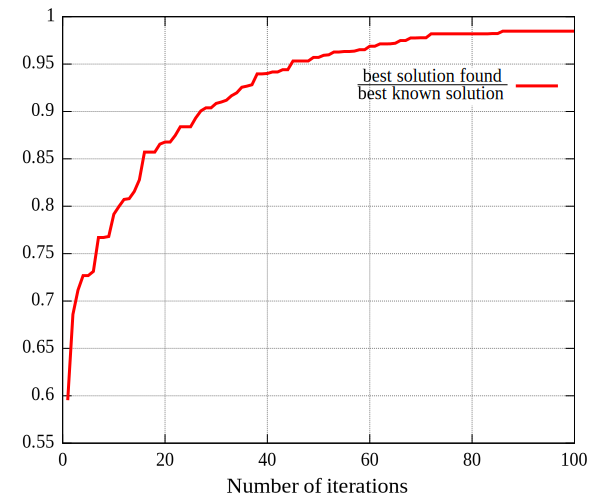
\includegraphics[scale=0.5]{imgs/iter}
  \caption{Convergence process of SCE for MKP
    for a problem with $n=500$, $m=30$ and $t=0.50$.}
  \label{fig:iter}
\end{figure}

The fast convergence speed of SCE for MKP can be noticed in Fig.~\ref{fig:iter}.
The figure shows for each iterations step, the quality of best solution found
for the first $100$ iterations.
The problem instance used was taken from the second set of problem (random instances).
The best known solution was found with $600$s of execution on SCIP solver and
the execution of the SCE algorithm expended $1.1$ seconds.

\section{Conclusions and future remarks}
\label{sec:conc}

In this work we addressed the application of the shuffled complex
evolution (SCE) to the multidimensional knapsack problem and investigated it
performance through several computational experiments.

The SCE algorithm, which combines the ideas of a controlled random search with
the concepts of competitive evolution proved to be very effective in finding
good solution for hard instances of MKP, demanding a very small amount of
processing time to reach high quality solutions for MKP.

Future work includes the investigation of different crossing procedures 
and the use of local search in the process of evolving complexes.

%\bibliographystyle{abbrv}
\bibliographystyle{IEEEtran}
\bibliography{../../refs}

%\printbibliography

\end{document}

